\باب{مویج اور گھمکیا}\شناخت{باب_مویج}
اب تک ہم صرف \اصطلاح{عرضی برقی و مقناطیسی}\فرہنگ{عرضی!برقی و مقناطیسی}\حاشیہب{transverse electromagnetic, TEM}\فرہنگ{transverse electromagnetic}\فرہنگ{TEM}  \تحریر{TEM} امواج کی بات کرتے آ رہے ہیں جن میں برقی اور مقناطیسی دونوں میدان سمت حرکت کے عمودی ہوتے ہیں۔اس باب میں ترسیلی تار پر بحث کو آگے بڑھاتے ہوئے ایسے امواج پر غور کیا جائے گا جن میں برقی یا مقناطیسی میدان سمت حرکت کی جانب بھی جزو رکھتے ہوں۔وہ ترسیلی تار جو صرف اس طرح کے امواج کو گزار سیکھیں \اصطلاح{میوج}\فرہنگ{مویج}\حاشیہب{waveguide}\فرہنگ{waveguide} کہلاتے ہیں۔

دو لامحدود جسامت کے مستوی سطحوں کے مویج سے بات شروع کرتے ہوئے کھوکھلے مستطیلی اور نلکی مویج تک بات بڑھائی جائے گی۔ان مویج میں میدان کے اشکال، ان کے منقطع طول موج اور تقلیلی مستقل  حاصل کئے جائیں گے۔اس کے بعد ایک تار پر بیرونی موج اور دیگر اقسام کے مویج پر غور کیا جائے گا۔آخر میں موصل کے بند ڈبوں میں قید امواج پر غور کیا جائے گا جنہیں گھمکیا کہتے ہیں۔

\حصہ{برقی دور، ترسیلی تار اور مویج کا موازنہ}
کم تعدد پر برقی دباو، برقی رو، مزاحمت وغیرہ عملی متغیر ہیں جنہیں استعمال کرتے ہوئے برقی ادوار حل کئے جاتے ہیں۔ان تعدد پر تمام مزاحمت یا رکاوٹ کو نقطہ نما تصور کیا جاتا ہے۔یوں تار کے ایک سرے پر منبع برقی دباو لاگو کرتے ہوئے تار کے دوسرے سرے پر مزاحمت میں برقی رو حاصل کی جا سکتی ہے۔

قدر زیادہ تعدد پر انہیں حقائق کو ترسیلی تار پر لاگو کیا جا سکتا ہے۔ایسا کرتے وقت ترسیلی تار کی مزاحمت یا امالہ تار کی لمبائی پر تقسیم شدہ  تصور کرنا لازم ہے۔ساتھ ہی ساتھ ترسیلی تار پر برقی دباو کی رفتار پر بھی نظر رکھنی ہوتی ہے۔

اب موصل کھوکھلے نلکی یا مستطیلی نالی پر مبنی نظام کی بات کرتے ہیں۔کیا ایسی نالی برقی و مقناطیسی طاقت منتقل کرنے کی صلاحیت رکھتی ہے؟ اگر ہماری معلومات برقی ادوار یا ترسیلی تار تک محدود ہوتی تب اس سوال کا جواب یہ ہے کہ ایسا ممکن نہیں ہے کیونکہ برقی طاقت کے منتقلی کے لئے دو تار ضروری ہیں۔البتہ اگر ہم شعاعوں کا علم رکھتے تب جواب ہوتا کہ ایسا ممکن ہے چونکہ شعاعیں سیدھی کھوکھلے نلکی سے گزر سکتی ہیں اور شعاعیں بلند تعدد \عددیء{(\SI{e16}{\hertz})} کی برقی و مقناطیسی امواج ہی ہیں۔

اصل جواب ہے کہ ایسا امواج کے تعدد پر منحصر ہے۔کم تعدد کے امواج نالی سے نہیں گزر سکتے جبکہ بلند تعدد کے امواج اس سے گزر سکتے ہیں۔تعدد کے ان دو خطوں کے درمیان ایسی تعدد ہو گی جس سے کم تعدد نالی سے نہیں گزرے گی اور جس سے زیادہ تعدد نالی سے گزرے گی۔اس تعدد کو \اصطلاح{پست انقطاعی تعدد}\فرہنگ{تعدد!پست انقطاعی}\فرہنگ{انقطاعی!پست تعدد}\حاشیہب{low cutoff frequency}\فرہنگ{frequency!low cutoff} کہا جاتا ہے۔ 

کھوکھلے نالی سے برقی و مقناطیسی طاقت کی منتقلی برقی ادوار حل کرنے کے علم سے ناقابل سمجھ مسئلہ ہے۔کھوکھلے نالی میں طاقت کی منتقلی، نالی کے کھوکھلے حصے میں برقی اور مقناطیسی میدان پر غور سے سمجھا جا سکتا ہے جنہیں استعمال کرتے ہوئے  پوئنٹنگ سمتیہ سے موج کی طاقت حاصل ہوتی ہے۔دراصل برقی و مقناطیسی طاقت نالی کے کھوکھلے حصے میں برقی اور مقناطیسی امواج سے منتقل ہوتا ہے نا کہ نالی کے موصل حصے میں۔برقی دباو اور برقی رو اس منتقلی کے محض اضافی اثرات ہیں۔ 

\حصہ{دو لامحدود وسعت کے مستوی چادروں کے مویج میں عرضی برقی موج}
شکل \حوالہ{شکل_مویج_لامحدود_متوازی_چادر} میں دو لامحدود وسعت کے متوازی چادروں پر مبنی ترسیلی تار دکھائی گئی ہے جو \عددیء{y} سمتی عرضی برقی و مقناطیسی موج گزار سکتی
 ہے۔ اس تار کی خاص خاصیت یہ ہے کہ ایک مخصوص تعدد کے اوپر یہ دیگر \اصطلاح{بلند درجی انداز}\فرہنگ{انداز!بلند درجی}\حاشیہب{higher order mode}\فرہنگ{mode!higher order} کے امواج بھی گزار سکتی ہے۔یوں ترسیلی تار سے شروع کرتے ہوئے مویج تک بحث کو پہنچانے  کے لئے یہ بہترین مثال ہے۔

\begin{figure}
\centering
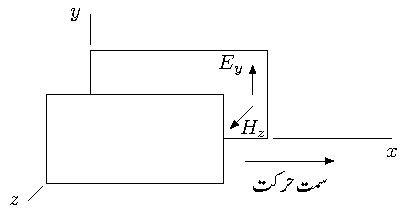
\includegraphics{figWaveguidesInfiniteParallelPlates}
\caption{دو لامحدود وسعت کے متوازی موصل چادروں کا نظام۔}
\label{شکل_مویج_لامحدود_متوازی_چادر}
\end{figure}

ایسی بلند درجی انداز کی بات کرتے ہیں جس میں برقی میدان ہر نقطے پر \عددیء{y} سمتی ہے جبکہ سمت حرکت \عددیء{\ax} ہے۔چونکہ برقی میدان سمت حرکت کے عمودی ہے لہٰذا اس انداز کو \اصطلاح{عرضی برقی انداز}\فرہنگ{عرضی!برقی انداز}\فرہنگ{انداز!عرضی برقی}\حاشیہب{transverse electric mode, TE mode}\فرہنگ{transverse electric mode}\فرہنگ{mode, transverse electric, TE} \تحریر{(TE)} کہا جائے گا۔اگرچہ اس موج میں برقی میدان عرضی ہے، مقناطیسی میدان عرضی اور طولی اجزاء پر مشتمل ہے۔کامل موصل چادروں کی صورت میں چادروں پر برقی میدان صفر ہو گا البتہ چادر سے دور  اس کی کچھ بھی قیمت ممکن ہے۔ایسی عرضی برقی انداز موج کے خصوصیات باآسانی یوں حاصل کئے جا سکتے ہیں کہ اسے دو عرضی برقی و مقناطیسی انداز \تحریر{TEM} امواج کا مجموعہ تصور کیا جائے جو موصل چادروں کے درمیان بار بار انعکاس کرتی ہوں۔

آئیں پہلے شکل \حوالہ{شکل_مویج_دو_عرضی_امواج_خالی_خلاء} پر غور کریں جہاں خالی خلاء میں ایک ہی تعدد کے دو سطحی \تحریر{TEM} امواج کے ملاپ کی صورت حال دکھائی گئی ہے۔اس شکل میں امواج خطی قطبی تصور کئے گئے ہیں جن کا برقی میدان صفحہ کے عمودی فرض کیا گیا ہے۔موج الف کی شعاع اوپر بائیں ہاتھ سے نیچے دائیں ہاتھ کی طرف جبکہ موج ب کی شعاع نیچے بائیں ہاتھ سے اوپر دائیں ہاتھ کی جانب گامزن ہے۔یوں ان کا آپس میں ملاپ کسی زاویے پر ہوتا ہے۔شکل میں گہری سیاہی کی ٹھوس لکیر سے موج کی چوٹی جبکہ ہلکی سیاہی کے ٹھوس لکیر سے اس کا نشیب دکھایا گیا ہے۔یوں سطحی موج الف کی چوٹیاں اور نشیب، شعاع الف کے عمودی دکھائے گئے ہیں۔گہری سیاہی کے ٹھوس لکیر کو برقی میدان کی چوٹی تصور کیا جائے۔یوں اس لکیر پر برقی میدان زیادہ سے زیادہ قیمت رکھتا ہے اور اس کی سمت صفحہ سے عمودی باہر جانب کو ہے۔اسی طرح ہلکی ٹھوس لکیر میدان کی نشیب کو ظاہر کرتی ہے لہٰذا یہاں میدان کی قیمت زیادہ سے زیادہ ہو گی البتہ اس کی سمت صفحہ کے عمودی اندر جانب کو ہو گی۔چوٹی اور نشیب کے درمیان فاصلہ \عددیء{\tfrac{\lambda_0}{2}} کے برابر ہے۔ 
%
\begin{figure}
\centering
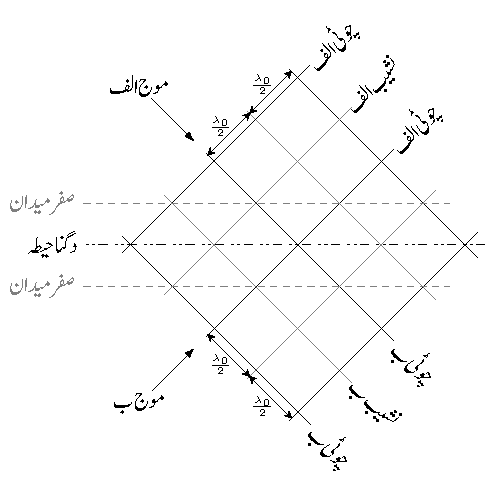
\includegraphics{figWaveguidesTwoIntersectingTEMwaves}
\caption{دو عرضی برقی و مقناطیسی امواج خلاء میں مختلف سمتوں میں حرکت کر رہی ہیں۔}
\label{شکل_مویج_دو_عرضی_امواج_خالی_خلاء}
\end{figure}

جس نقطے پر ایک موج کی چوٹی اور دوسری موج کا نشیب ملتے ہیں اس نقطے پر کل میدان صفر کے برابر ہو گا۔یوں جہاں گہری سیاہی اور ہلکی سیاہی کے لکیر ملتے ہیں وہاں میدان صفر ہو گا۔شکل میں ہلکی سیاہی میں ایسی دو نقطہ دار لکیریں کھینچی گئی ہیں جن پر میدان صفر کے برابر ہے۔آپ غور کر کے تسلی کر لیں کہ ان لکیروں کے ہر نقطے پر برقی میدان صفر ہی ہے۔مزید آپ ذہن میں دونوں امواج کو حرکت دیتے ہوئے تسلی کر لیں کہ امواج کے حرکت کے باوجود ان دو لکیروں پر میدان صفر ہی رہتا ہے۔اسی طرح جن نقطوں پر دونوں امواج کی چوٹیاں آپس میں ملتی ہوں یا دونوں کے نشیب آپس میں ملتے ہوں وہاں میدان دگنا ہو گا۔شکل میں ہلکی سیاہی اور دو نقطوں والی ایسی ایک عدد  لکیر دکھائی گئی ہے جہاں میدان دگنا پایا جائے گا۔

صفر میدان دکھاتے نقطہ دار لکیر پر برقی میدان صفر کے برابر ہے لہٰذا ان پر موصل سطح کے سرحدی برقی میدان کا شرط پورا اترتا ہے۔یوں ان لکیروں پر، صفحہ کے عمودی  موصل چادر رکھے جا سکتے ہیں۔البتہ ایسا کرنے سے موج کی سیدھی حرکت متاثر ہو گی چونکہ آمدی زاویے کے برابر، موصل سطح پر، انعکاسی زاویے سے موج انعکاس کرے گی۔یوں موج موصل سطح سے گزر نہیں پائے گی۔ہاں اگر دو موصل چادروں کے درمیان ان امواج کو بھیجا جائے، تب یہ دونوں موصل سطحوں کے درمیان بار بار انعکاس کرتی حرکت کریں گی۔شکل \حوالہ{شکل_مویج_شعاع_انعکاس_کرتی_حرکت_کرتی_ہے} میں ایسا دکھایا گیا ہے۔ شکل \حوالہ{شکل_مویج_خالی_خلاء_اور_میوج_طول-موج} میں مویج میں موج کی چوٹی اور نشیب دکھائے گئے ہیں۔خالی خلاء میں طول موج اور مویج میں طول موج کا تعلق بھی دکھایا گیا ہے۔ 

\begin{figure}
\centering
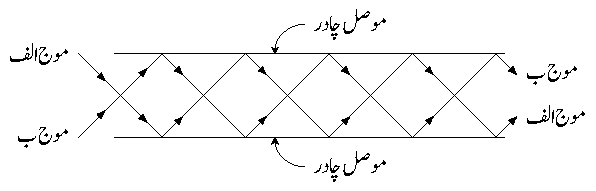
\includegraphics{figWaveguidesTwoConductingSheetsTwoTEMwaves}
\caption{شعاعیں دو چادروں کے درمیان بار بار انعکاس کرتی حرکت کرتی ہیں۔}
\label{شکل_مویج_شعاع_انعکاس_کرتی_حرکت_کرتی_ہے}
\end{figure}
%
\begin{figure}
\centering
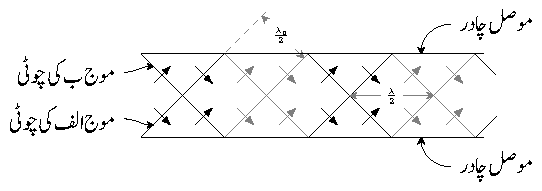
\includegraphics{figWaveguidesTwoConductingSheetsTwoTEMwavesWavefronts}
\caption{موجوں کی چوٹیاں، نشیب، خالی خلاء اور مویج میں طول موج۔}
\label{شکل_مویج_خالی_خلاء_اور_میوج_طول-موج}
\end{figure}
